\documentclass[border=12pt]{standalone}
\def\pgfsysdriver{pgfsys-dvisvgm.def}
\usepackage[dvisvgm]{xcolor}
\usepackage{xeCJK}
\setCJKmainfont{HaranoAjiGothic-Regular.otf}[BoldFont=HaranoAjiGothic-Bold.otf]
\setCJKsansfont{HaranoAjiGothic-Regular.otf}[BoldFont=HaranoAjiGothic-Bold.otf]
\usepackage{amsmath,amssymb,tikz,lmodern}
\usetikzlibrary{arrows.meta,positioning,calc,fit,backgrounds}
\renewcommand{\familydefault}{\sfdefault}
\definecolor{ink}{HTML}{25322F}
\definecolor{green}{HTML}{246657}
\definecolor{tint}{HTML}{EEF4F0}
\definecolor{soft}{HTML}{C6D2CC}
\definecolor{muted}{HTML}{52615B}
\newif\ifJapanese
\newcommand{\Tx}[2]{\ifJapanese #1\else #2\fi}
\newcommand{\Eff}{\overline{\operatorname{Eff}}}
\newcommand{\heading}[3]{{\color{green}\bfseries #1\quad\Tx{#2}{#3}}\\[5pt]}
% A white rectangle makes the complete citation label clickable, including spaces.
\newcommand{\refurl}[2]{\special{dvisvgm:raw <a xlink:href="#1" target="_blank" rel="noopener noreferrer">}{\setlength{\fboxsep}{0pt}\colorbox{white}{\color{green}\underline{\strut #2}}}\special{dvisvgm:raw </a>}}
\newcommand{\refedge}[3]{\refurl{\csname source#1\endcsname\string##page=#2}{#3}}
\newcommand{\SF}[2]{\refedge{sf}{#1}{#2}}
% GitHub's file preview does not support PDF page fragments.
\newcommand{\LA}[2]{\refurl{\sourcela}{#2}}
\newcommand{\Sch}[2]{\refedge{sch}{#1}{#2}}
\newcommand{\PS}[2]{\refedge{ps}{#1}{#2}}
\tikzset{
 card/.style={draw=soft,fill=white,rounded corners=2pt,align=left,text=ink,font=\fontsize{10.5}{14}\selectfont,inner xsep=12pt,inner ysep=10pt,text width=14.4cm},
 half/.style={card,text width=6.45cm,minimum height=2.05cm},
 result/.style={card,draw=green,fill=tint,line width=.9pt},
 reason/.style={align=left,text=muted,font=\fontsize{9}{12}\selectfont,inner sep=0pt,text width=12.7cm},
 branchreason/.style={reason,text width=5.95cm},
 edge/.style={-{Stealth[length=2.4mm]},draw=green,line width=1pt},
 wire/.style={draw=green,line width=1pt},
}
% Keep the arrow in a dedicated left gutter; explanations never cover it.
\newcommand{\flow}[3]{
 \coordinate (#2-from) at ($(#1.south)+(-6.9,0)$);
 \coordinate (#2-to) at ($(#2.north)+(-6.9,0)$);
 \draw[edge] (#2-from)--(#2-to);
 \node[reason,anchor=west] (#2-reason) at ($(#2-from)!.5!(#2-to)+(.55,0)$) {#3};
}
\newcommand{\Cite}[2]{\refurl{\csname source#1\endcsname}{#2}}

\Japanesetrue
\newcommand{\sourceslc}{https://github.com/openai/math/blob/adc7f1241b42e322a6451854ab7e4b4c146bf78a/preprints/Uniform-indices-for-semi-log-canonical-log-Calabi-Yau-pairs-October-5-2026/uniform-slc-index.pdf}
\newcommand{\sourceui}{https://github.com/openai/math/blob/adc7f1241b42e322a6451854ab7e4b4c146bf78a/preprints/Uniform-Pluricanonical-Iitaka-Fibrations-October-3-2026/paper.pdf}
\newcommand{\sourcela}{https://github.com/openai/math/blob/adc7f1241b42e322a6451854ab7e4b4c146bf78a/preprints/Log-abundance-in-characteristic-zero-September-24-2026/paper.pdf}
\newcommand{\sourceuli}{https://github.com/openai/math/blob/adc7f1241b42e322a6451854ab7e4b4c146bf78a/preprints/Uniform-log-Iitaka-fibrations-and-bounded-moduli-denominators-October-4-2026/uniform-log-iitaka.pdf}
\newcommand{\sourcek}{https://arxiv.org/pdf/1107.2863v3}
\newcommand{\sourcehj}{https://arxiv.org/pdf/2204.04946v2}
\newcommand{\sourcejl}{https://arxiv.org/pdf/2002.11928}
\begin{document}
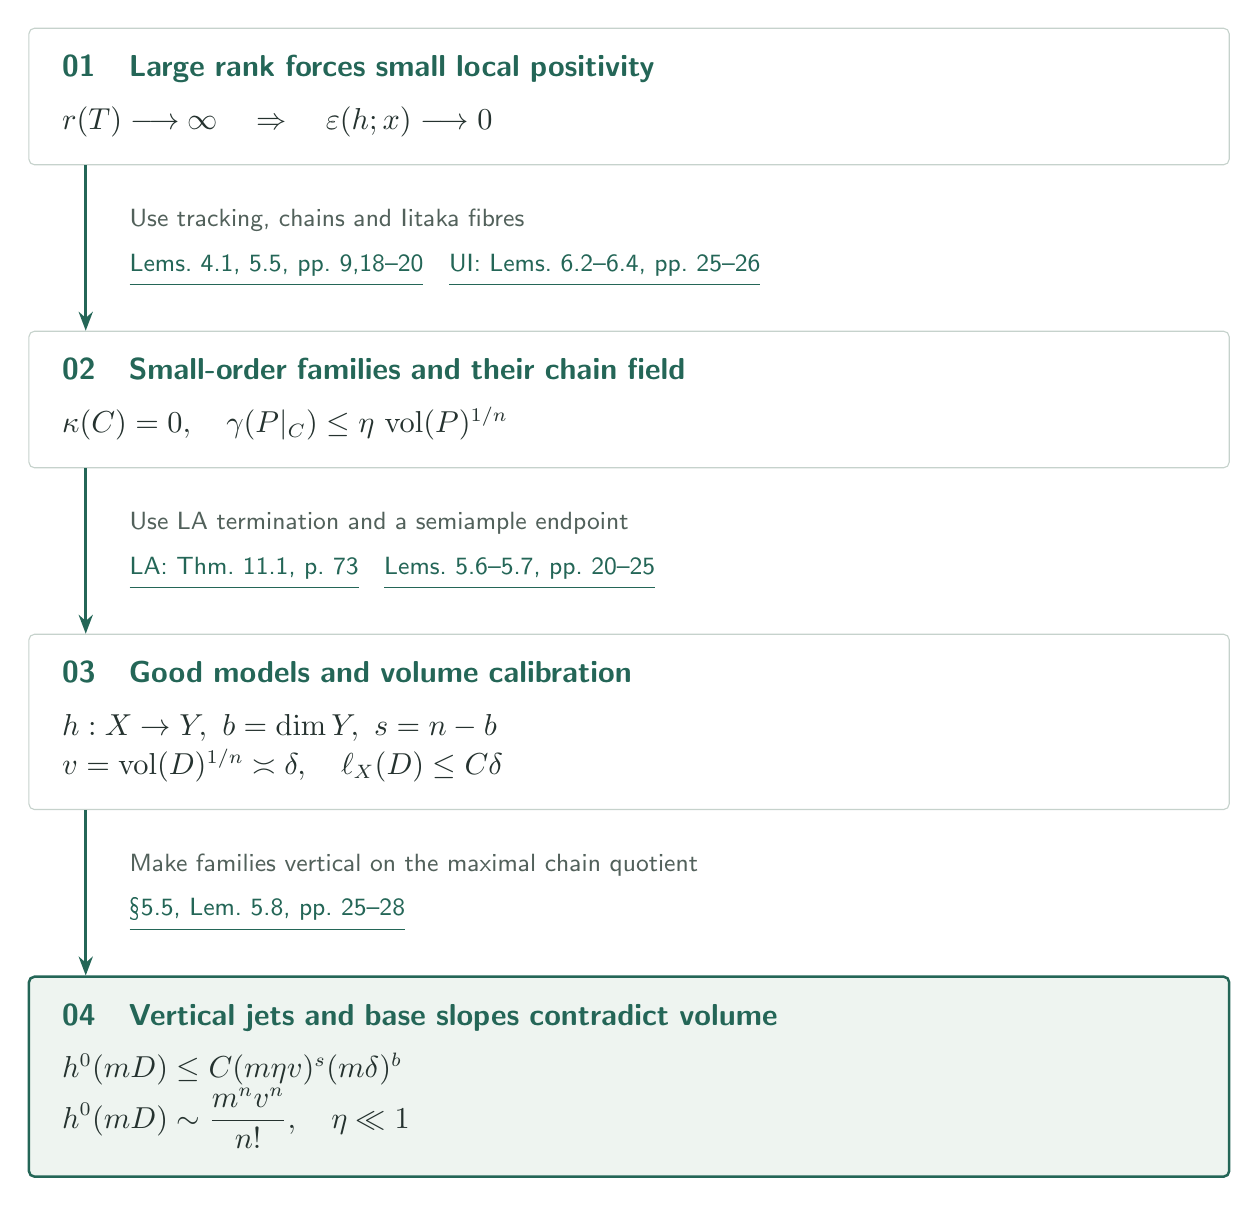
\begin{tikzpicture}
\node[card] (n0) {\heading{01}{大きいrankから小さい局所正値性へ}{Large rank forces small local positivity}\Tx{$r(T)\longrightarrow\infty\quad\Rightarrow\quad\varepsilon(h;x)\longrightarrow0$}{$r(T)\longrightarrow\infty\quad\Rightarrow\quad\varepsilon(h;x)\longrightarrow0$}};
\node[card,below=2.1cm of n0] (n1) {\heading{02}{小消滅次数の族とchain field}{Small-order families and their chain field}\Tx{$\kappa(C)=0,\quad \gamma(P|_C)\leq\eta\,\operatorname{vol}(P)^{1/n}$}{$\kappa(C)=0,\quad \gamma(P|_C)\leq\eta\,\operatorname{vol}(P)^{1/n}$}};
\flow{n0}{n1}{\Tx{tracking・chain・Iitaka fibreで次元を下げる}{Use tracking, chains and Iitaka fibres}\\[4pt]\Cite{slc}{Lems.\ 4.1, 5.5, pp.\ 9,18--20}\quad \Cite{ui}{UI: Lems.\ 6.2--6.4, pp.\ 25--26}}
\node[card,below=2.1cm of n1] (n2) {\heading{03}{良いモデルと体積の較正}{Good models and volume calibration}\Tx{$h:X\to Y,\ b=\dim Y,\ s=n-b$\\$v=\operatorname{vol}(D)^{1/n}\asymp\delta,\quad\ell_X(D)\leq C\delta$}{$h:X\to Y,\ b=\dim Y,\ s=n-b$\\$v=\operatorname{vol}(D)^{1/n}\asymp\delta,\quad\ell_X(D)\leq C\delta$}};
\flow{n1}{n2}{\Tx{LAの停止・semiample終点を実際に使う}{Use LA termination and a semiample endpoint}\\[4pt]\Cite{la}{LA: Thm.\ 11.1, p.\ 73}\quad \Cite{slc}{Lems.\ 5.6--5.7, pp.\ 20--25}}
\node[result,below=2.1cm of n2] (n3) {\heading{04}{垂直jetと底の傾きから矛盾}{Vertical jets and base slopes contradict volume}\Tx{$h^0(mD)\leq C(m\eta v)^s(m\delta)^b$\\$\displaystyle h^0(mD)\sim \frac{m^nv^n}{n!},\quad \eta\ll1$}{$h^0(mD)\leq C(m\eta v)^s(m\delta)^b$\\$\displaystyle h^0(mD)\sim \frac{m^nv^n}{n!},\quad \eta\ll1$}};
\flow{n2}{n3}{\Tx{最大chain quotientで族を垂直にする}{Make families vertical on the maximal chain quotient}\\[4pt]\Cite{slc}{\S5.5, Lem.\ 5.8, pp.\ 25--28}}
\end{tikzpicture}
\end{document}
